\documentclass[preprint,10pt]{elsarticle}

\usepackage{amssymb}
\usepackage{amsmath}
\usepackage{lineno}
\usepackage{hyperref}

\usepackage{epstopdf}
\usepackage{epsfig}
\usepackage{setspace}

\newcommand{\be}{\begin{equation}}
\newcommand{\ee}{\end{equation}}
\newcommand{\beq}{\begin{eqnarray}}
\newcommand{\eeq}{\end{eqnarray}}
\newcommand{\ba}{\begin{eqnarray}}
\newcommand{\ea}{\end{eqnarray}}

\newcommand{\ua}{{\bf u}_\alpha}
\newcommand{\utwo}{\overline{\bf u}_2}
\setcounter{MaxMatrixCols}{24}

\journal{Coastal Engineering}

\begin{document}


%\title{Model derivations}

\begin{center}
{\bf \Large Nesting FUNWAVE in a large-scale wave-averaged model}
 \end{center}
 
 \section{The idea }
 
 Nesting FUNWAVE in a large-scale wave-averaged model has three steps
 
 \noindent
 1) interpolate the results $(u,v,\eta)$, from the large-scale model into the FUNWAVE grid. 
 
 As shown in Figure \ref{two_grid}, the output region(grid point, red dots ) of the large-scale model should cover the entire FUNWAVE grid, which avoids any extrapolation. The grid of the large-scale model should be a structured grid, either curvilinear or rectangular grid. Values at $A$ are obtained from interpolations within the angle (1,2,3) marked in the Figure (see detailed in the next section). 
 
 \noindent
 2) incorporate the large-scale model results into the sponge layer
 
 Figure \ref{sponge} shows sponge layers for example. The sponge layers can be configured in any of the four boundaries. In the current case, WEST, SOUTH, and NORTH sponges are specified. 
 
 \noindent
 3) make waves at the wavemaker location
 
 An internal wavemaker should be used for this application. The west boundary wavemaker CANNOT be used due to the application of the WEST sponge. 
 
  \begin{figure}
\begin{center}
 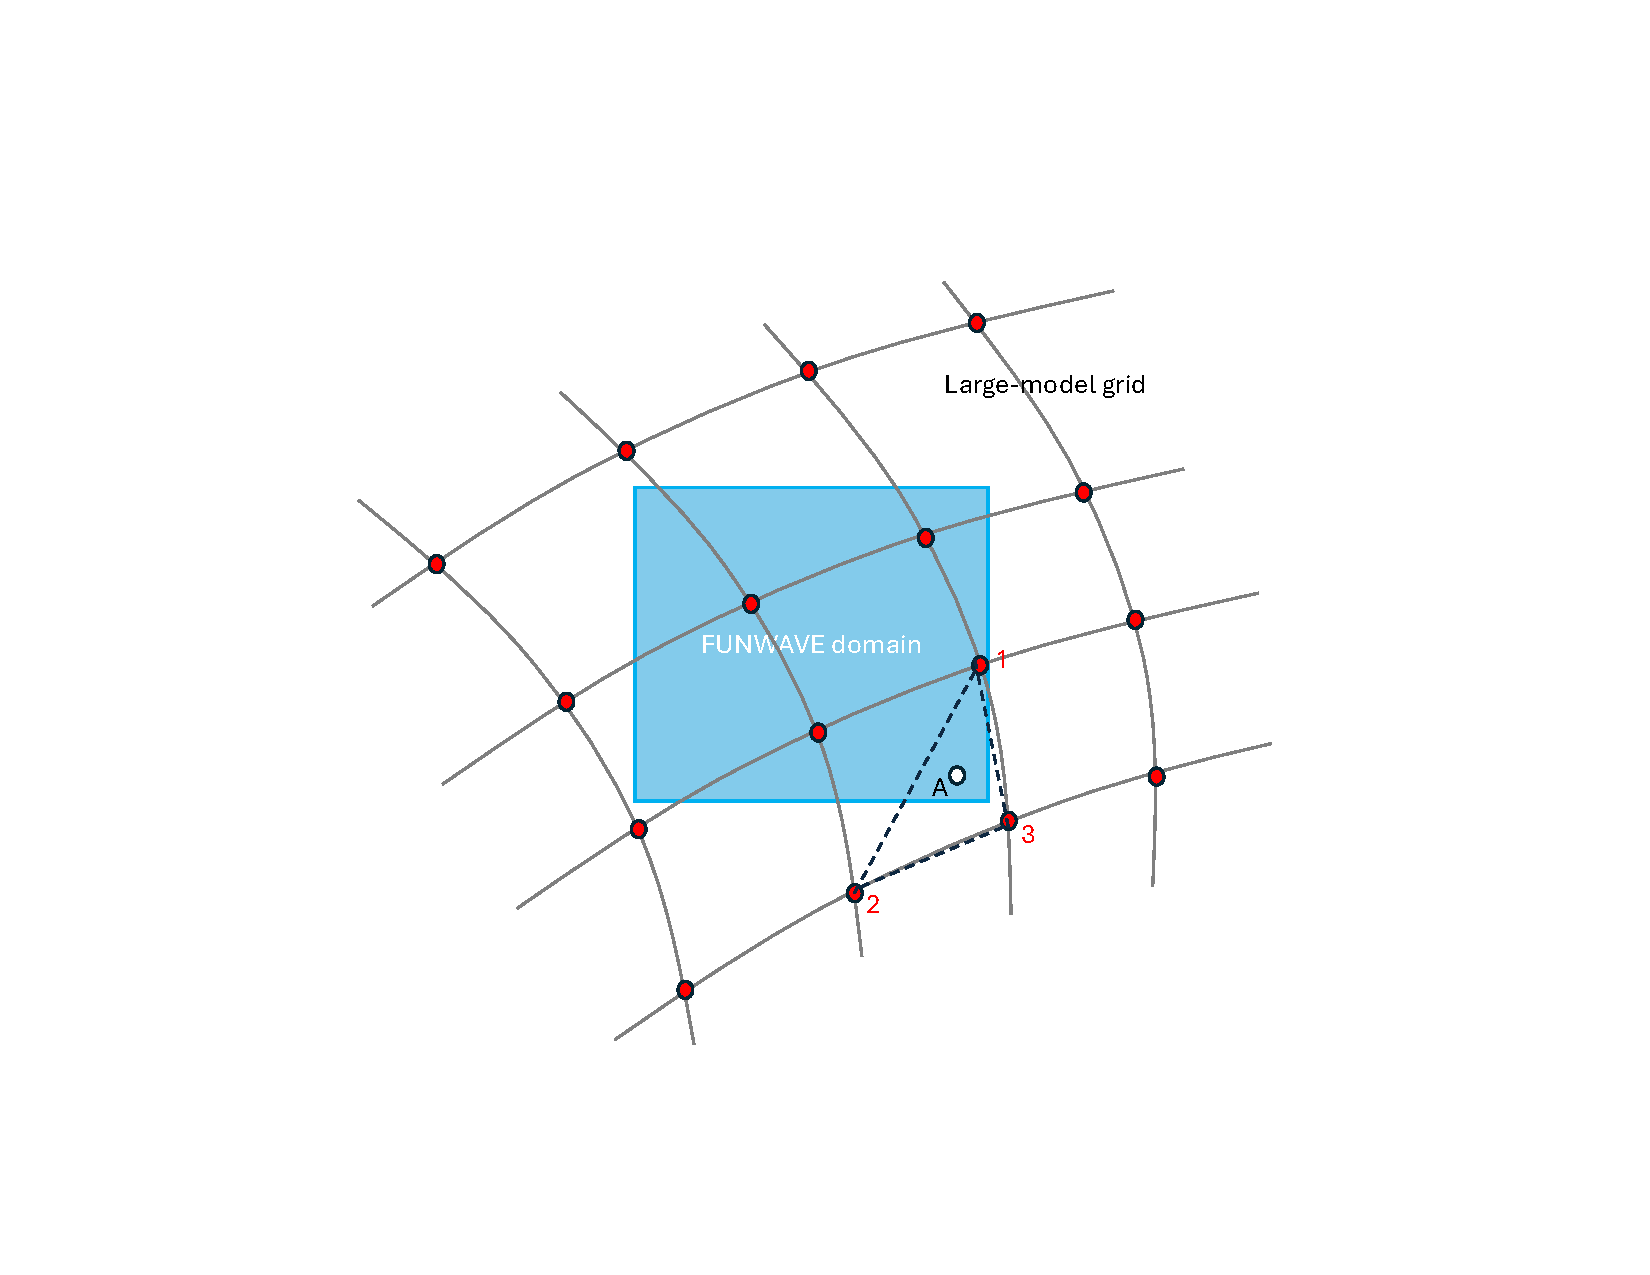
\includegraphics[width=1.0\textwidth]{figures/two_grids.pdf}
 \caption{Interpolation triangle }
 \label{two_grid}
 \end{center}
 \end{figure}
 
  \begin{figure}
\begin{center}
 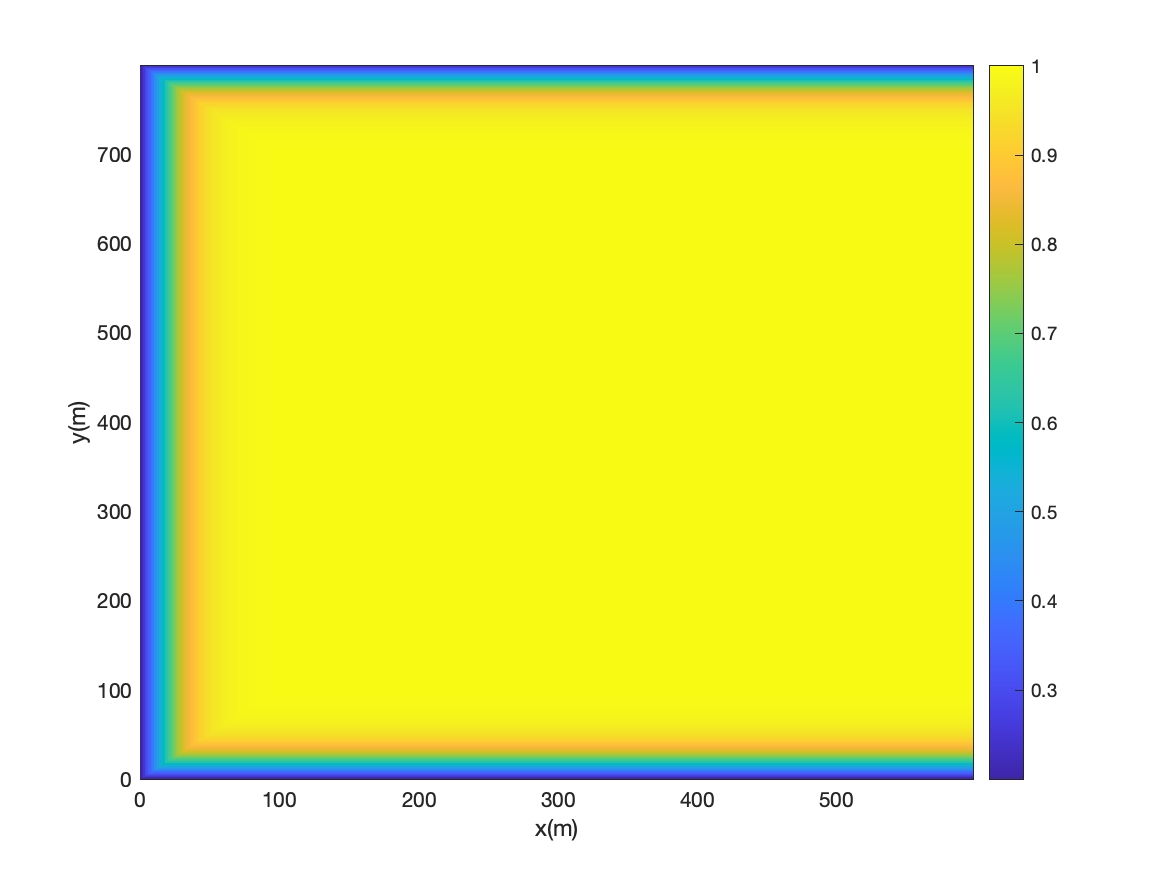
\includegraphics[width=1.0\textwidth]{figures/sponge_2d.jpg}
 \caption{2D sponge layers }
 \label{sponge}
 \end{center}
 \end{figure}
 
 \section{Interpolation} 
  
  Interpolation or extrapolation (not suggested) is  employed between a structured grid of a large-scale model
 and the FUNWAVE grid.  A linear interpolation method is performed.
As shown in Figure \ref{triangle}, an interpolation
value at  point $A$ in the FUNWAVE grid is evaluated by the values at three points, $1,
2$ and $3$, of a triangle in the large-scale model grid which surrounds point $A$.  Four triangle areas
$S_{\alpha \beta \gamma}$, i.e., $S_{123}, S_{12A}, S_{31A}$ and $S_{23A}$ are
calculated using the following formula:
  
\ba
S_{\alpha \beta \gamma}=\left | \begin{array}{ccc}x_\alpha & y_\alpha & 1 \\
x_\beta & y_\beta & 1 \\
x_\gamma & y_\gamma &1 
\end{array}
\right |
\ea
where $(x_{\alpha}, y_{\alpha}$) represents
coordinates of point $1, 2, 3$ and $A$.  For interpolation, ($\alpha, \beta,
\gamma$) are  counter-clockwise for all the four triangles and thus $S_{\alpha
\beta \gamma}$ are positive. For extrapolation, clockwise ($\alpha, \beta,
\gamma$) results in negative $S_{\alpha
\beta \gamma}$. The following formula is used for both interpolation and
extrapolation:
\be
F_A=(F_1S_{23A}+F_2 S_{31A} + F_3 S_{12A})/S_{123}
\ee
where $F_1, F_2, F_3$ and $F_A$ represent any converted variables at
point $1, 2, 3 $ and $A$, respectively.

To save computational time for interpolation/extrapolation, $S_{\alpha
\beta \gamma}$ values are stored in the initialization stage (only calculated once).  
  
 \begin{figure}
\begin{center}
 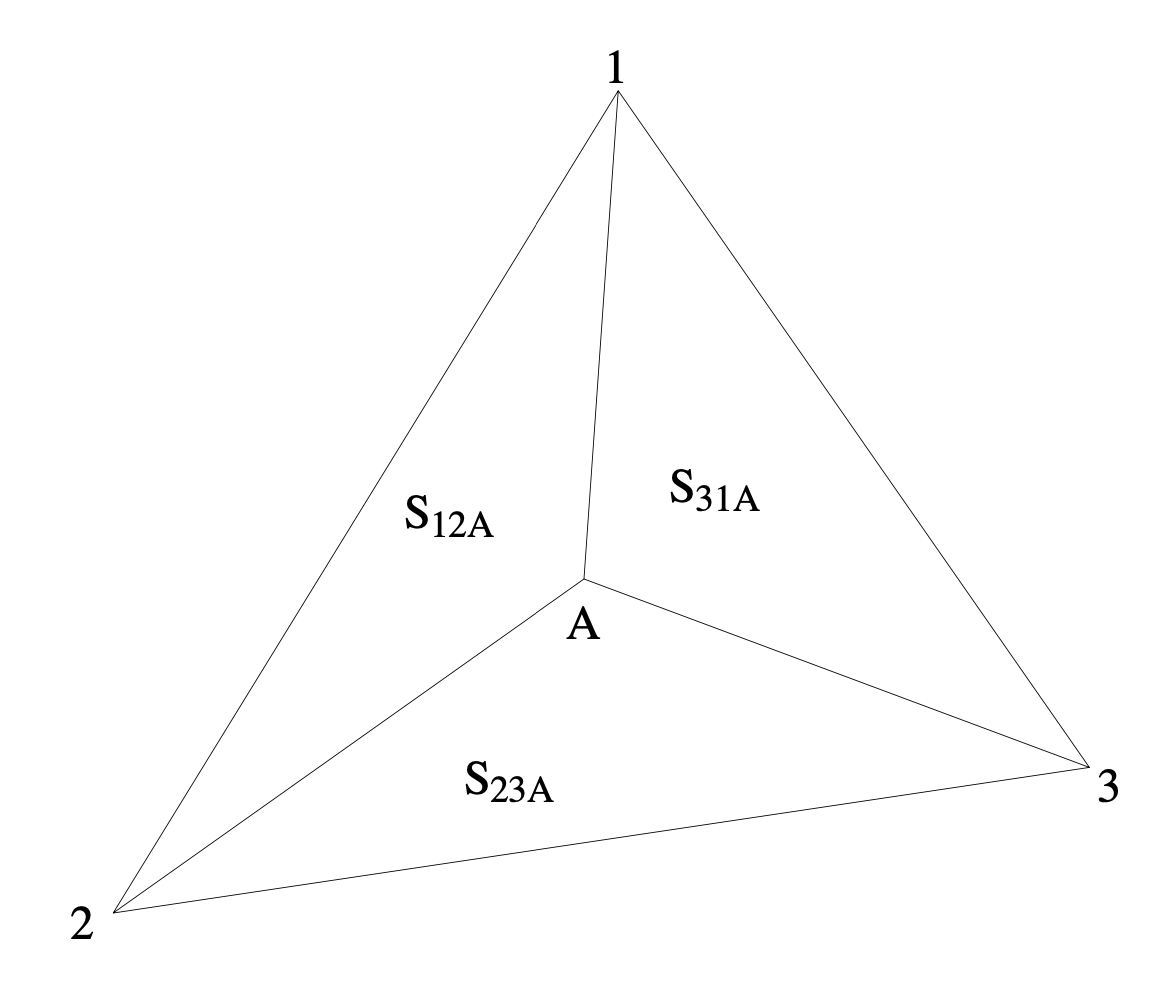
\includegraphics[width=1.0\textwidth]{figures/triangle.png}
 \caption{Interpolation triangle }
 \label{triangle}
 \end{center}
 \end{figure}
  

\section{The new module}
   
 The new module is called  `ABS\_GEN\_2D\_MODULE' in mod\_2d\_abs\_gen.F. To activate this module, you should specify 
 
  -DMAP2D\_ABS\_GEN
  
  in Makefile when compiling the the code. In input.txt, the following parameters are needed, for example
  
 \noindent 
MAP2D\_GEN\_ABS = T \\
BC\_WEST\_NEST = T \\
BC\_EAST\_NEST = F \\
BC\_SOUTH\_NEST = T  \\
BC\_NORTH\_NEST = T  \\
MappingDataFileName = large\_model\_data.txt   
 
In the application,  BC\_EAST\_NEST = F is applied, meaning no sponge and large-scale model results are needed. The nesting boundary conditions will be applied on WEST, SOUTN, and NORTH boundaries. 

large\_model\_data.txt contains the large-scale model results in time. The following is an example of the data format:

\vspace{0.5cm}
\noindent
eta, u, v data from a large-scale model (void line) \\
2 2 ! M\_DATA N\_DATA (the data grid is 2x2) \\
! 2d x-coordinate (void line) \\
0 1000  (x-coordinates)\\
0 1000  (x-coordinates)\\
! 2d y-coordinate (void line)\\
0 0  (y-coordinates)\\
1200 1200 (y-coordinates) \\
0.0   -time (in second) \\
0.0 0.0 - eta \\
0.0 0.0 \\
0.0 0.0  - u \\
0.0 0.0 \\
0.0  0.0 - v \\
0.0 0.0  \\
500.0   -time \\
0.5 0.1 - eta \\
0.0 0.0 \\
0.0 0.0  - u \\
0.0 0.0 \\
0.0 0.0 - v \\
0.0 0.0  

   
\section{Example}

The example can be found in /nest\_large\_model/. Procedures:

1) compile and code in the example folder

2) check input.txt

3) run the model

4) matlab scripts can be found in /postprocessing/

The following are two plots from the example. 

 \begin{figure}
\begin{center}
 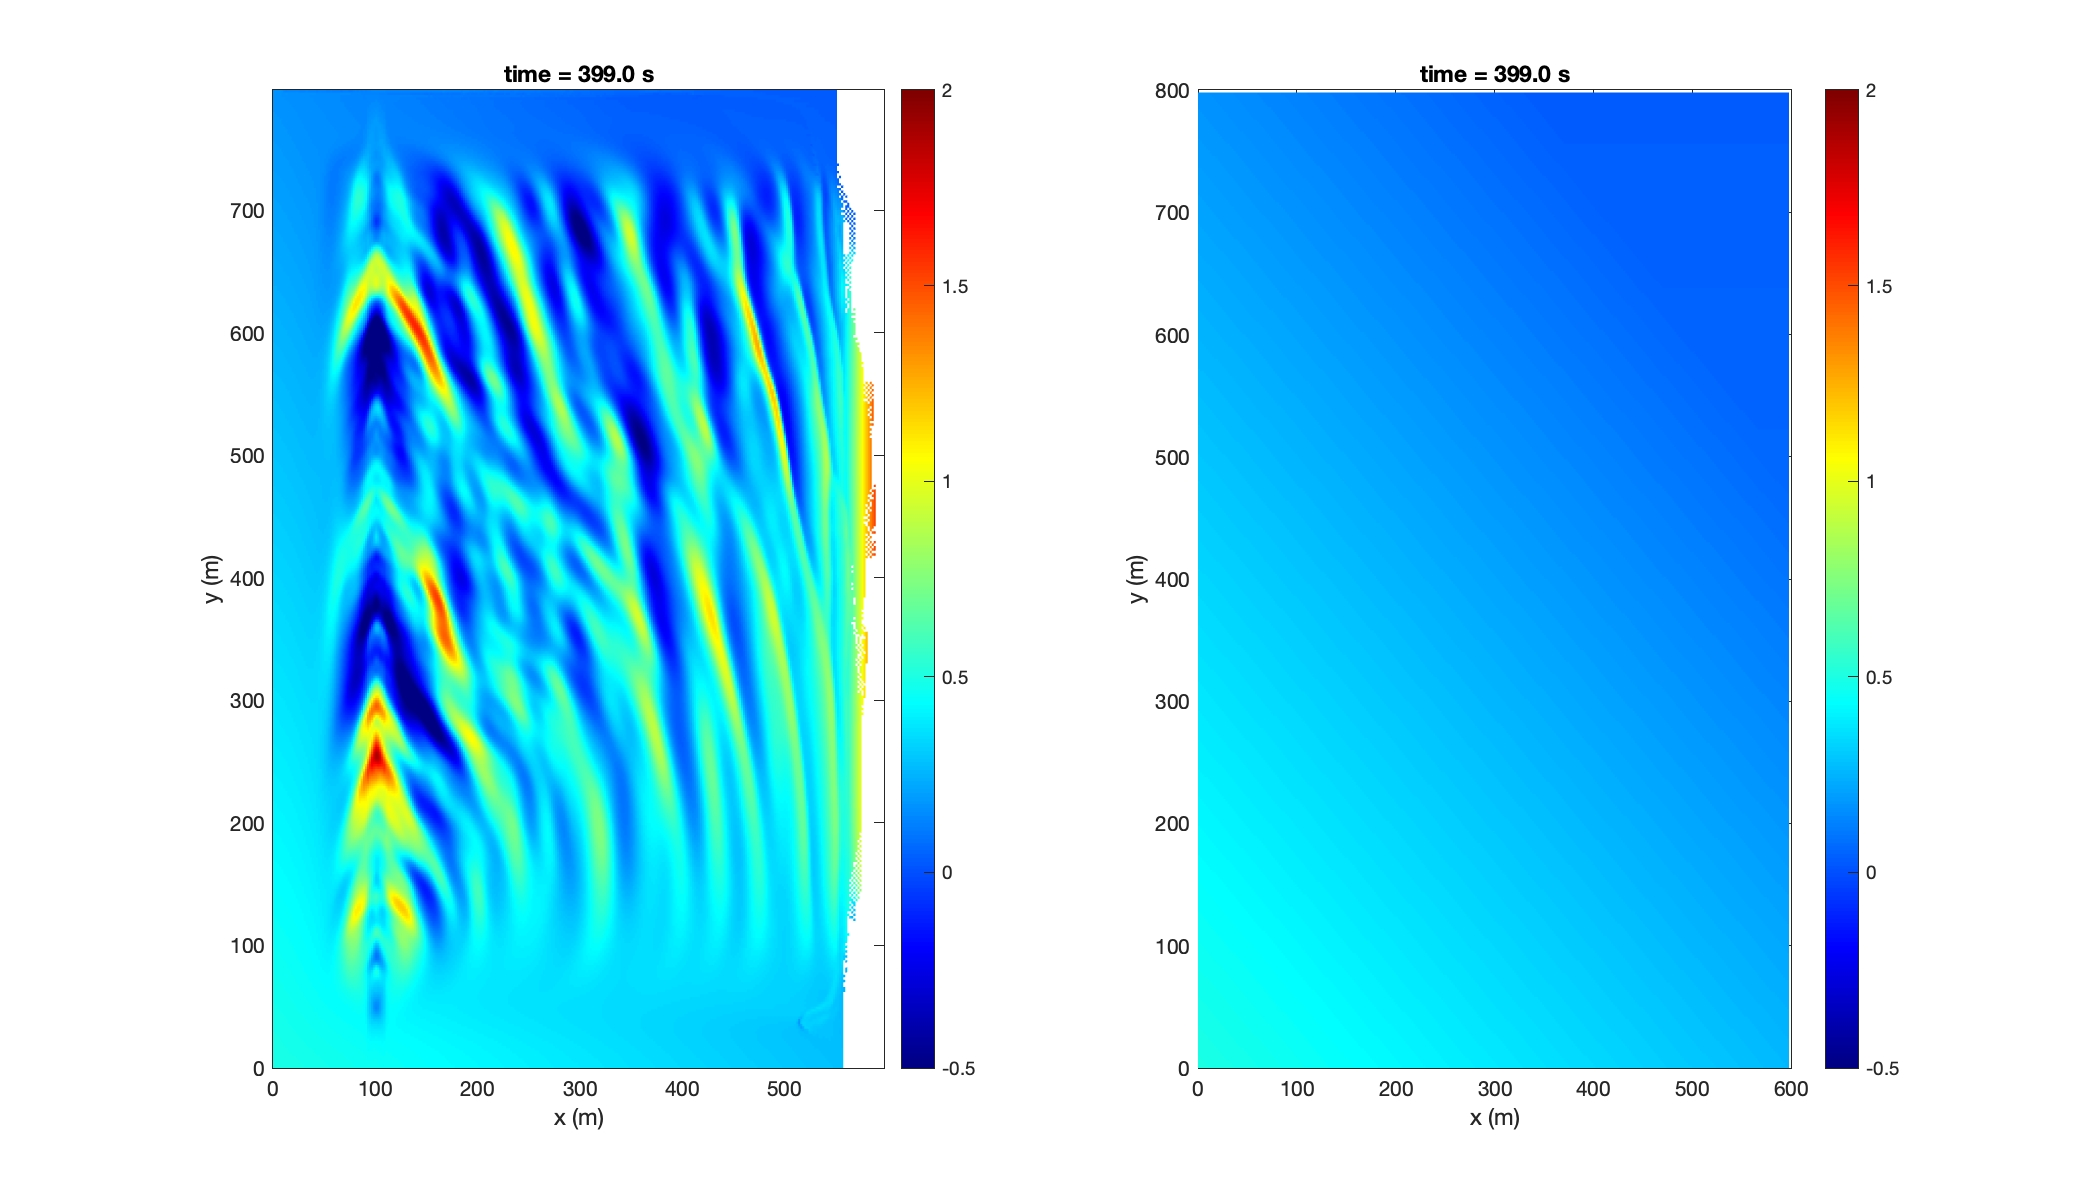
\includegraphics[width=1.0\textwidth]{figures/elevation_view.jpg}
 \caption{Left: surface elevation from FUNWAVE; right: surface elevation interpolated from the large-scale model }
 \label{surface}
 \end{center}
 \end{figure}  
  
  \begin{figure}
\begin{center}
 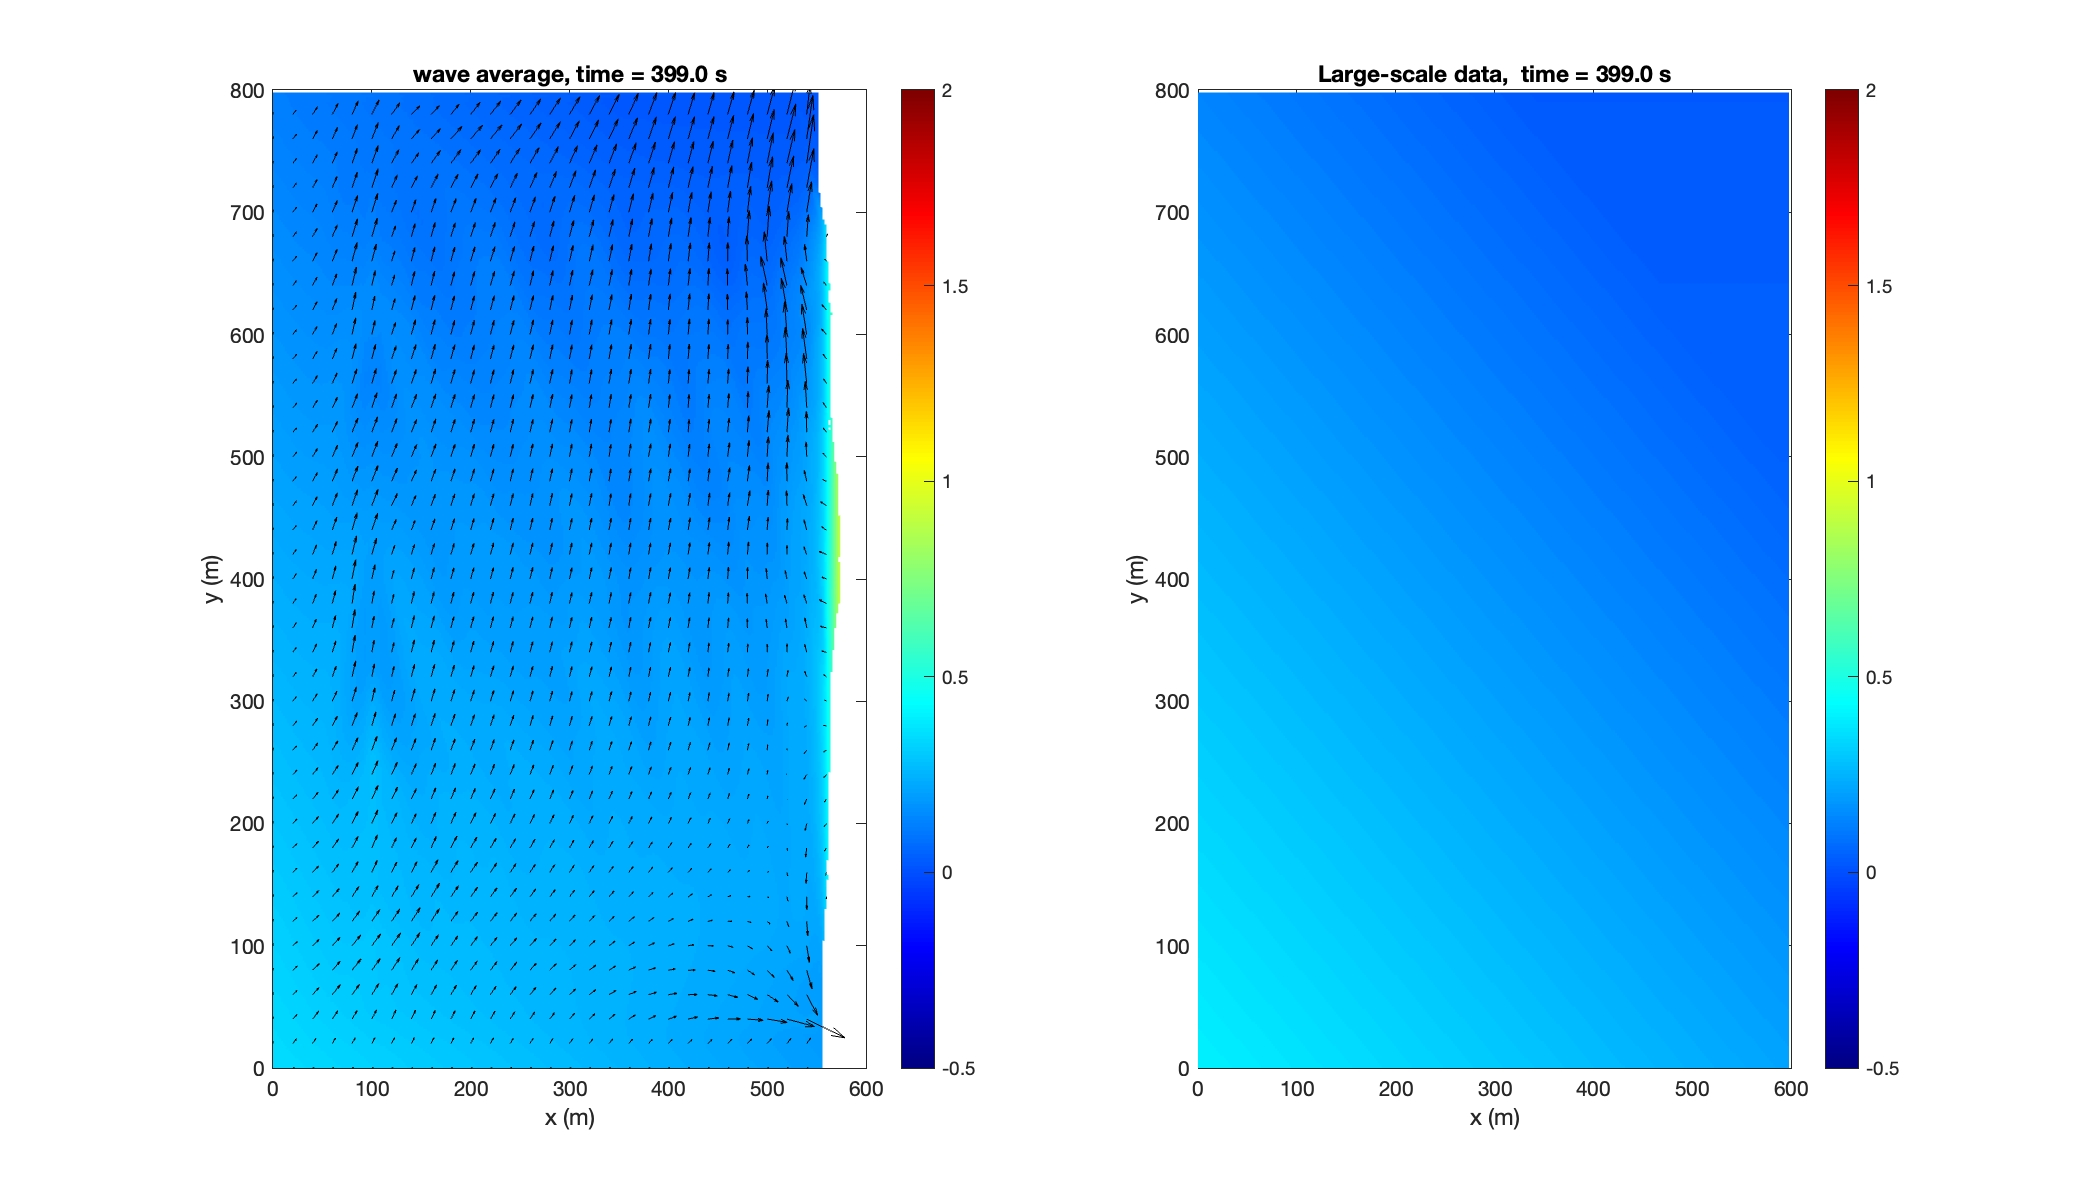
\includegraphics[width=1.0\textwidth]{figures/uvmean_view.jpg}
 \caption{Left: mean surface and mean velocity from FUNWAVE; right: surface elevation interpolated from the large-scale model }
 \label{mean}
 \end{center}
 \end{figure}  
  
\end{document}







